\chapter{Related Work}
%Add some context information and introduction before delving into the related work.

Web-based/Computer based education and adaptive web-based assessment systems are a ``hot" research area, and as a result, numerous tools, environments and infrastructures have emerged. There are common features to all, however some distinguish themselves by having not so common features.
Automated exercise generation in these tools is usually non-existent or very limited. Moreover, the tools are more focused on assessing students rather than self-assessment, i.e. students take tests which count towards their final grade on these systems.\newline

There are many components involved in this project, two of the more important ones are adaptive difficulty and automated generation of exercises, so there are many tools which exist which do one or the other, very rarely both.\newline

In this section we look at related software and evaluate them with respect to the objectives listed at the beginning of the development of jSCAPE.

\section{Environment for Learning to Program}
Environment for Learning to Program (ELP) is an interactive web based environment for teaching programming to first year Information Technology students at Queensland University of Technology (QUT).

\section{CourseMarker}
CourseMarker is a re-design of Ceilidh, a computer based assessment system used at the University of Nottingham for 13 years. Ceilidh was quite a complete system, providing coursework, the management of modules and the presentation of module content.

\section{Automatic Exercise Generator with Tagged Documents based on the Intelligence of Students}
The Automatic Exercise Generator with Tagged Documents based on the Intelligence of Students (AEGIS)

\section{Programming Adaptive Testing}
\begin{figure}[H]
\centering
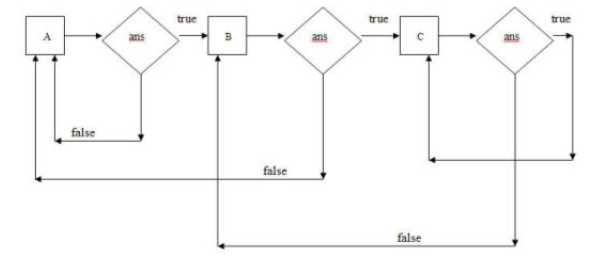
\includegraphics[width=\textwidth,height=\textheight,keepaspectratio]{PAT_adaptive_sequence}
\caption{Adaptive sequence of questions in PAT. (Source:\cite{PAT})}
\label{fig:PAT_adaptive_sequence}
\end{figure}

\section{Adaptive Self-Assessment Master}
Adaptive Self-Assessment Master (ASAM) is an extension to CourseMarker, which improves upon it by administering questions which are suited to the student's ability.

\section{System of Intelligent Evaluation Using Tests for Tele-education}
The System of Intelligent Evaluation Using Tests for Tele-education (SIETTE) is a web based environment for generating and constructing adaptive tests.

\section{Summary}
We have looked at some of the relevant work in the field of computer based education and assessment. We saw that SIETTE provided many of the features we set out to replicate in jSCAPE, therefore particular parts of our implementation will be inspired by SIETTE.